\section{Machine Learning}
The already mentioned neural networks belong to a wider field of machine learning (ML) - the study of using experience to improve algorithms. This section assumes a basic understanding of ML and gives a brief overview of the topics needed to understand the scope of the project. It then explains in more details the background and related work for the architectures involved in this research.


\subsection{Classification accuracy, Area-Under-Curve, and confusion matrix} \label{ml-accuracy-auc-confusion}
There are several key metrics used for assessing the success of an ML algorithm, and the following will be used throughout the report:

\begin{itemize}
  \item \textbf{Classification accuracy} - a simple measure of the percentage of correctly classified samples.
  \item \textbf{Confusion matrix} - a tabular metric that compares the actual samples' classes with the predicted ones, effectively categorizing results into four groups: true positive, false positive, false negative, and true negative. This allows for an easy calculation of precision and recall values.
  \item \textbf{Area Under the Curve (AUC) for the Receiver Operator Characteristic (ROC)} - a more complex measure of the model's ability to correctly distinguish between classes. It can be used similarly to the classification accuracy, but it favors discriminative over representative models.
\end{itemize}


\subsection{Deep Neural Networks}
While there exist a number of ML techniques that have proven successful for various use cases at LHC, like Support Vector Machines \cite{38-valentino2012classification} or Boosted Decision Trees \cite{pmlr-v42-chen14}, in the last years deep neural networks (DNN) have been proposed with improved results for applications like infrastructure monitoring \cite{39-skoczen2016lstm}, offline data analysis \cite{40-ren2020unveiling}, and the main interest of this report - detectors' trigger mechanisms.

In many uses cases the neural networks architectures are optimized and accelerated to shorten the training time (often measured in hours) to reduce the time needed for evaluating different design configurations and easily perform the hyperparameter search. However, this work focuses on accelerating the inference to match the extremely low latency required in the LHC detectors' L1 triggers. Although often measured in milliseconds, sub-milliseconds inference time has been achieved for this application with the use of FPGAs using architectures for basic DNN \cite{36-kreinar2018fast}, and recently sub-microseconds latency for graph neural networks (GNN) \cite{42-kreinar2020distance-weighted, 41-elabd2021graph}. These implementations serve as a baseline latency for this project which aims to achieve comparable performance with higher AUC value. A commonality between the recent best performing designs is the use of the \textit{hls4ml} codesign workflow that was mentioned in \autoref{motivation}.

\subsection{Transformer Neural Networks and Attention}
A promising architecture that has been chosen as the first implementation for this project is the transformer neural network, which is a type of recurrent neural network (RNN). A recent implementation \cite{3-yuan2021constituentnet:} called ConstituentNet outperforms previous state-of-the-art graph neural networks (GNN) implementations like JEDI-net \cite{9-newman2019jedi-net:} using a version of the attention mechanism \cite{44-vaswani2017attention}, called self-attention. A diagram with a high-level view of the ConstituentNet can be seen in figure \ref{fig:constituent-net}.

\begin{figure}[hpt!]
  \centering
  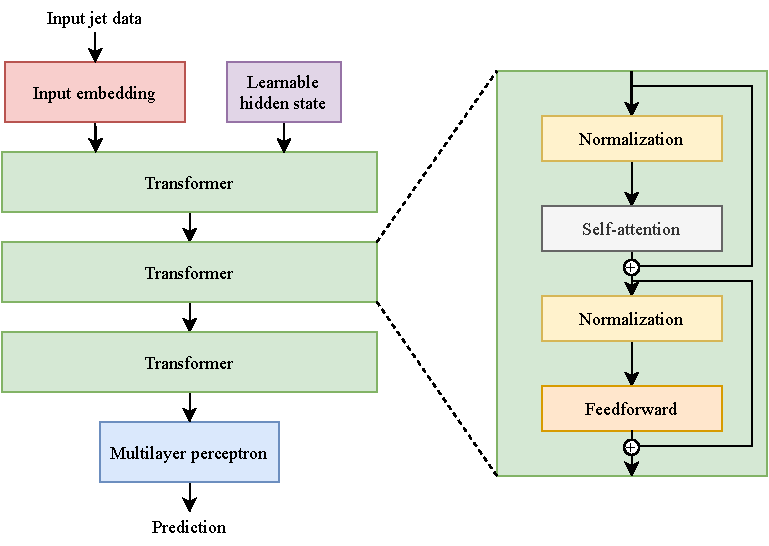
\includegraphics[trim={0cm 0cm 0cm 0cm}, width=0.6\textwidth, center]{background/constituent_net.pdf}
  \caption{High-level overview of the ConstituentNet architecture}
  \label{fig:constituent-net}
\end{figure}

Given the strong results of its software implementation, an FPGA-mapped design can become an improvement over existing designs for L1Ts at LHC. A number of techniques are planned to ensure the design matches the required performance, which includes quantization and pruning \cite{45-liang2021pruning} and careful exploration of the trade-off between latency and hardware resource utilization, which is covered in \autoref{latency-throughput-resources}.


\subsection{Dataset}
The datasets used in this work has been obtained from the 13 TeV proton-proton collisions performed at LHC, and it includes information about the most energetic jets \cite{31-pierinihls4ml,32-pierinihls4ml,33-pierinihls4ml,34-pierinihls4ml} that were constructed using the anti-K\textsubscript{t} clustering algorithm \cite{35-cacciari2008anti-kt}. A number of representations are available in the dataset and the one used for this project contains lists of jets' constituent hadrons from the following list: light quarks, top quarks, W bosons, Z bosons, and gluons.


